\documentclass[tikz,border=12pt]{standalone}
\usepackage[T1]{fontenc}
\usepackage{tgheros}
\usepackage{sfmath}
\usepackage{amsmath,amssymb}
\usepackage{fontawesome5}
\usepackage{tikz}
\usetikzlibrary{arrows.meta,positioning,shapes.geometric,fit,backgrounds,calc}
\usepackage{xcolor}

\renewcommand{\familydefault}{\sfdefault}

% Canonical Semantic Palette
\definecolor{structuralnavy}{HTML}{1B2A4A}
\definecolor{measuredteal}{HTML}{168F84}
\definecolor{proposalamber}{HTML}{C98218}
\definecolor{consequencecoral}{HTML}{BD4F2F}
\definecolor{authorityviolet}{HTML}{6550A8}
\definecolor{neutralgray}{HTML}{687386}
\definecolor{navyfill}{HTML}{E8EDF6}
\definecolor{tealfill}{HTML}{E4F6F3}
\definecolor{amberfill}{HTML}{FFF3DC}
\definecolor{coralfill}{HTML}{FAE9E2}
\definecolor{grayfill}{HTML}{F4F6F7}
\definecolor{cardborder}{HTML}{CBD5E1}

\begin{document}
\begin{tikzpicture}[
  font=\sffamily,
  >=Stealth,
  card/.style={
    draw=cardborder,
    fill=white,
    rounded corners=5pt,
    line width=0.8pt,
    inner sep=8pt
  }
]

  % Title banner
  \node[card, fill=navyfill, draw=structuralnavy, text width=7.4in, align=left] (header) {
    \textbf{\color{structuralnavy}\faIcon{tachometer-alt}\; THE THREE SPEEDS OF PHYSICAL AI INTELLIGENCE} \hfill {\scriptsize\color{neutralgray} Cadence Hierarchy \& Execution Substrates}
  };

  % Row 1: The 3 Speeds
  \node[card, draw=authorityviolet, fill=white, text width=2.12in, below=0.20in of header.south west, anchor=north west, minimum height=1.60in] (c_sys2) {
    {\color{authorityviolet}\textbf{\faIcon{brain}\; System 2: Deliberation}}\\[2pt]
    {\scriptsize\textbf{Cadence:} $0.5\text{--}2\text{ Hz}$ ($500\text{--}2000\text{ ms}$)}\\[3pt]
    {\footnotesize\textbf{Substrate:} Cloud / Host Linux MPU}\\[2pt]
    {\footnotesize\textbf{Function:} Semantic parsing, open-vocabulary 3D grounding, expiring intent leases ($t_{\text{expire}}$).}\\[3pt]
    {\scriptsize\color{neutralgray}\mbox{OpenVLA} $\cdot$ \mbox{LLaVA-OneVision} $\cdot$ \mbox{GPT-4o}}
  };

  \node[card, draw=proposalamber, fill=amberfill!25, text width=2.12in, right=0.52in of c_sys2, minimum height=1.60in] (c_sys15) {
    {\color{proposalamber}\textbf{\faIcon{network-wired}\; System 1.5: Planning}}\\[2pt]
    {\scriptsize\textbf{Cadence:} $15\text{--}50\text{ Hz}$ ($20\text{--}66\text{ ms}$)}\\[3pt]
    {\footnotesize\textbf{Substrate:} Embedded SoC NPU / GPU}\\[2pt]
    {\footnotesize\textbf{Function:} Trajectory generation, multi-step action chunking ($H=16$), temporal ensembling.}\\[3pt]
    {\scriptsize\color{neutralgray}\mbox{Diffusion Policy} $\cdot$ \mbox{ACT} $\cdot$ \mbox{Flow Matching}}
  };

  \node[card, draw=measuredteal, fill=white, text width=2.12in, right=0.52in of c_sys15, minimum height=1.60in] (c_sys1) {
    {\color{measuredteal}\textbf{\faIcon{shield-alt}\; System 1: Reflex}}\\[2pt]
    {\scriptsize\textbf{Cadence:} $1000\text{ Hz}$ ($1\text{ ms}$)}\\[3pt]
    {\footnotesize\textbf{Substrate:} Bare-Metal / FreeRTOS MCU}\\[2pt]
    {\footnotesize\textbf{Function:} Real-time CBF invariants, spline evaluation, dynamic stopping veto, PWM timer registers.}\\[3pt]
    {\scriptsize\color{neutralgray}\mbox{ARM Cortex-M4/M7} $\cdot$ \mbox{STM32} $\cdot$ \mbox{CBF-QP}}
  };

  % Connecting Arrows with Badges
  \draw[->, line width=1.0pt, authorityviolet, dashed] (c_sys2.east) -- (c_sys15.west)
    node[midway, above=2pt, font=\tiny\bfseries, fill=white, draw=authorityviolet!40, rounded corners=2pt, inner sep=2pt] {3D Lease ($t_{\text{expire}}$)};
  
  \draw[->, line width=1.2pt, proposalamber, dashed] (c_sys15.east) -- (c_sys1.west) 
    node[midway, above=2pt, font=\tiny\bfseries, fill=white, draw=proposalamber!40, rounded corners=2pt, inner sep=2pt] {Chunk $A_t$ ($H=16$)};

  % Row 2: Latency Starvation vs Action Chunking Timeline Container
  \coordinate (tl_top) at ($(c_sys2.south west) + (0, -0.22in)$);

  % Outer background box
  \draw[draw=cardborder, fill=grayfill!30, rounded corners=5pt, line width=0.8pt] 
    (tl_top) rectangle ++(7.68in, -3.9in);

  \node[anchor=north west, font=\small\bfseries, color=structuralnavy] at ($(tl_top) + (0.15in, -0.12in)$) {
    \faIcon{history}\; Latency Starvation vs. Action Chunk Delay Amortization
  };

  % ----------------------------------------------------
  % PANEL A: Single-Step Failure
  % ----------------------------------------------------
  \coordinate (pa_header) at ($(tl_top) + (0.2in, -0.40in)$);
  \node[anchor=north west, font=\footnotesize\bfseries, color=consequencecoral] at (pa_header) {
    A. Single-Step Markovian Policy ($H=1$) $\implies$ Discrete Latency Starvation \& Mechanical Chatter
  };

  \coordinate (pa_base) at ($(pa_header) + (0.1in, -0.75in)$);

  % Time Axis A
  \draw[->, line width=0.7pt, neutralgray] (pa_base) -- ++(4.6in, 0) node[right, font=\scriptsize] {Time ($t$)};
  \foreach \x/\label in {0/0, 1.0/20, 2.0/40, 3.0/60, 4.0/80} {
    \draw[neutralgray] ($(pa_base) + (\x in, 2pt)$) -- ($(pa_base) + (\x in, -2pt)$) 
      node[below, font=\tiny] {\label$\text{ ms}$};
  }

  % Inference 1 (0 to 50ms = 2.5in)
  \draw[draw=proposalamber, fill=amberfill, line width=0.7pt, rounded corners=2pt]
    ($(pa_base) + (0, 0.08in)$) rectangle ++(2.5in, 0.28in)
    node[midway, font=\tiny\bfseries, color=proposalamber] {Inference 1 ($50\text{ ms}$)};

  % Step 1 execution at 50ms (takes 1ms = 0.05in)
  \draw[draw=consequencecoral, fill=coralfill, line width=0.8pt]
    ($(pa_base) + (2.5in, 0.08in)$) rectangle ++(0.12in, 0.28in);
  \node[above=2pt, font=\tiny\bfseries, color=consequencecoral] at ($(pa_base) + (2.56in, 0.36in)$) {Step 1};

  % Starvation 1 (51ms to 100ms)
  \draw[draw=consequencecoral!80, fill=coralfill!30, dashed, line width=0.6pt]
    ($(pa_base) + (2.62in, 0.08in)$) rectangle ++(1.88in, 0.28in)
    node[midway, font=\tiny\bfseries, color=consequencecoral] {\faIcon{exclamation-triangle}\; Starvation ($49\text{ ms}$)};

  % Inference 2 (starts at 50ms, ends at 100ms)
  \draw[draw=proposalamber, fill=amberfill, line width=0.7pt, rounded corners=2pt]
    ($(pa_base) + (2.5in, -0.42in)$) rectangle ++(2.0in, 0.24in)
    node[midway, font=\tiny\bfseries, color=proposalamber] {Inference 2 ($50\text{ ms}$)};

  % Side takeaway A
  \node[anchor=west, font=\scriptsize, align=left, color=consequencecoral] at ($(pa_base) + (5.1in, 0.05in)$) {
    \textbf{Gearbox Damage:}\\Motor jerks $1\text{ ms}$, freezes $49\text{ ms}$,\\exciting structural resonance.
  };

  % ----------------------------------------------------
  % PANEL B: Action Chunking
  % ----------------------------------------------------
  \coordinate (pb_header) at ($(tl_top) + (0.2in, -2.10in)$);
  \node[anchor=north west, font=\footnotesize\bfseries, color=measuredteal] at (pb_header) {
    B. Action Chunking ($H=16$, $K=8$) $\implies$ Delay Amortization \& Continuous $1\text{ kHz}$ Trajectory
  };

  \coordinate (pb_base) at ($(pb_header) + (0.1in, -0.75in)$);

  % Time Axis B
  \draw[->, line width=0.7pt, neutralgray] (pb_base) -- ++(4.6in, 0) node[right, font=\scriptsize] {Time ($t$)};
  \foreach \x/\label in {0/0, 1.0/20, 2.0/40, 3.0/60, 4.0/80} {
    \draw[neutralgray] ($(pb_base) + (\x in, 2pt)$) -- ($(pb_base) + (\x in, -2pt)$) 
      node[below, font=\tiny] {\label$\text{ ms}$};
  }

  % Chunk 1 Inference (0 to 50ms)
  \draw[draw=proposalamber, fill=amberfill, line width=0.7pt, rounded corners=2pt]
    ($(pb_base) + (0, 0.08in)$) rectangle ++(2.0in, 0.28in)
    node[midway, font=\tiny\bfseries, color=proposalamber] {Infer Chunk 1 ($A^{(0)}$)};

  % Chunk 1 Execution Stream (50ms to 90ms)
  \draw[draw=measuredteal, fill=tealfill, line width=0.8pt, rounded corners=2pt]
    ($(pb_base) + (2.0in, 0.08in)$) rectangle ++(1.2in, 0.28in)
    node[midway, font=\tiny\bfseries, color=measuredteal] {\faIcon{check-circle}\; Chunk 1 ($1\text{ kHz}$)};

  % Overlapped Chunk 2 Inference
  \draw[draw=proposalamber, fill=amberfill, line width=0.7pt, rounded corners=2pt]
    ($(pb_base) + (2.0in, -0.42in)$) rectangle ++(1.5in, 0.24in)
    node[midway, font=\tiny\bfseries, color=proposalamber] {Infer Chunk 2 ($A^{(1)}$)};

  % Chunk 2 Ensemble Blend
  \draw[draw=structuralnavy, fill=tealfill!50!amberfill!50, line width=0.8pt, rounded corners=2pt]
    ($(pb_base) + (3.2in, 0.08in)$) rectangle ++(1.3in, 0.28in)
    node[midway, font=\tiny\bfseries, color=structuralnavy] {\faIcon{random}\; Ensemble Blend};

  % Side takeaway B
  \node[anchor=west, font=\scriptsize, align=left, color=measuredteal] at ($(pb_base) + (5.1in, 0.05in)$) {
    \textbf{Zero Starvation:}\\Fluid $\mathcal{C}^2$ motion via\\overlapping chunk horizons.
  };

\end{tikzpicture}
\end{document}
